\chapter{روش پیشنهادی}
در این مقاله برای حل مسئله پیدا کردن استراتژی تخلیه بهینه یک سیستم رایانش لبه‌ای مطابق با شکل \ref{fig-offloading-system} در نظر می‌گیریم.
\begin{figure}[H]
	\centering
	\includegraphics*[width=\textwidth]{figures/MEC5.png}
	\caption{ساختار کلی سیستم تخلیه پردازش}
	\label{fig-offloading-system}
\end{figure}
\newpage
همانطور که در شکل \ref{fig-offloading-system} مشاهده می‌شود، در سامانه مد نظر سه مولفه اصلی زیر وجود دارد:
\begin{enumerate}
	\item دستگاه کاربر (\lr{User Equipment})
	\item سرور پردازش لبه‌ای چند-دسترسی (\lr{Multi-access Edge Computing Server})
	\item کانال بیسیم
\end{enumerate}
در فصل جاری ابتدا نحوه مدل‌سازی هر کدام از این مولفه‌ها شرح داده می‌شود و در انتها الگوریتم و ساختار نرم‌افزاری جدیدی ارائه می‌شود که می‌توان با استفاده از آن استراتژی تخلیه بهینه را به ازای یک سیستم داده شده محاسبه کرد.
\section{مدل وظایف}
فرض می‌شود که \(k\) نوع وظیفه مختلف در سیستم رایانش لبه‌ای وجود دارد و به ازای هر نوع وظیفه دقیقا یک صف در سیستم موجود است. وظایف نوع \(i\)-اُم برای اجرا به صورت محلی\LTRfootnote{Local} احتیاج به \(L_i\) بازه زمانی پردازش توسط واحد پردازنده دارند و به منظور تخلیه به سرور رایانش لبه‌ای احتیاج به \(M_i\) واحد زمانی ارسال توسط واحد ارسال\LTRfootnote{Transmission Unit} دارند. علاوه بر این فرض می‌شود که وظایف نوع \(i\)-اُم در سرور رایانش لبه‌ای به \(C_i\) بازه زمانی پردازش توسط سرور دارند. در ادامه این مقاله برای اشاره به یک واحد زمانی اجرا توسط پردازنده از عبارت \textbf{«قسمت»}\LTRfootnote{Section} استفاده می‌کنیم که انتزاعی از قسمت‌های کد اجرایی است. و برای اشاره به یک واحد زمانی ارسال توسط واحد ارسال از عبارت\textbf{ «بسته» }استفاده می‌شود.
\newpage
\section{مدل دستگاه کاربر}
\label{sec:ue-model}
دستگاه کاربر مطابق با شکل \ref{fig-offloading-system} شامل دو مولفه پردازنده و واحد ارسال می‌باشد. همچنین همانطور که اشاره شد \(k\) صف مختلف به ازای هر کدام از انواع وظایف در سیستم وجود دارد. ظرفیت هر صف را برابر با مقدار ثابت \(Q\) در نظر می‌گیریم. \\

در هر بازه زمانی، واحد پردازنده یا به اندازه یک قسمت پردازش انجام می‌دهد و یا بیکار\LTRfootnote{Idle} است. اجرای هر قسمت پردازش توسط پردازنده به میزان \(P_loc\) توان مصرف می‌کند. به طور مشابه واحد ارسال در هر بازه زمانی یا یک بسته را به شبکه ارسال می‌کند یا بیکار است. نکته قابل توجه در مورد واحد ارسال این است که با توجه به شرایط کانال بیسیم، در یک بازه زمانی خاص ممکن است ارسال موفقیت آمیز باشد یا نباشد. فرض می‌شود که ارسال موفقیت آمیز هر بسته به میزان \(P_tx\) توان مصرف می‌کند. توضیحات بیشتر در مورد نحوه کارکرد کانال بی‌سیم در بخش \ref{sec:wireless} آورده شده است. \\

با توجه به توضیحات داده شده می‌توان مدلی برای «حالت دستگاه کاربر»\LTRfootnote{User Equipment State} تعریف کرد. در مقاله \cite{Liu} برای مشخص کردن حالت دستگاه در زمان \(t\) از یک سه تایی مانند $\boldsymbol{\tau}[t]=\left(q[t], c_{T}[t], c_{L}[t]\right)$ استفاده شده است، که در آن \(q[t]\) مشخص کننده تعداد وظایف موجود در صف وظایف، \(c_T[t]\) مشخص کننده اندیس بسته ارسالی توسط واحد ارسال، و \(c_L[t]\) مشخص کننده اندیس قسمت\LTRfootnote{Section} اجرایی توسط پردازنده است. همچنین حالت \(c_T[t] = 0\) را معادل با بیکار بودن واحد ارسال و \(c_L[t] = 0\) را معادل بیکار بودن واحد پردازنده تعریف می‌کنیم. به عنوان نمونه سه تایی \((4, 2, 1)\) به این معنی است که ۴ وظیفه در صف وظایف وجود دارد، واحد پردازش در حال تخلیه وظیفه‌ای است و تا کنون یک بسته از آن وظیفه را ارسال کرده و به عنوان قدم بعدی باید بسته شماره ۲ را ارسال کند. واحد پردازنده نیز در حال اجرای وظیفه‌ای به صورت محلی است و تا کنون یک قسمت از آن وظیفه را اجرا کرده است. \\
\newpage
با این حال مدل فوق برای مسئله تخلیه وظایف ناهمگون قابل استفاده نیست و نیاز به تغییر دارد. ما در این مقاله برای تعیین حالت دستگاه کاربر از یک چندتایی\LTRfootnote{Tuple} به طول \(k + 4\) مطابق با رابطه \ref{eg:state} استفاده می‌کنیم. در این رابطه متغیرهای \(q_1[t]\) تا \(q_k[t]\) تعداد وظایف موجود از هر یک انواع وظیفه را در صف مربوطه مشخص می‌کنند. متغیرهای \(c_R[t]\) و \(c_L[t]\) مشابه مقاله \cite{Liu} تعریف می‌شوند و به ترتیب وضعیت واحد ارسال و واحد پردازنده را مشخص می‌کنند. دو متغیر جدید \(T_R[t]\) و \(T_L[t]\) به ترتیب مشخص کننده نوع وظیفه در حال ارسال توسط واحد ارسال و نوع وظیفه در حال اجرا توسط پردازنده اند.

\begin{equation}
	\label{eg:state}
	\tau[t]=\left(q_{1}[t], q_{2}[t], \ldots, q_{k}[t], c_{R}[t], c_{L}[t], T_{R}[t], T_{L}[t]\right)
\end{equation}
رابطه \ref{eq:state-space} شروط حاکم بر متغیرهای فضای حالت مسئله را عنوان می‌کند و به عبارتی توصیف‌گر فضای حالت مسئله است. \textbf{(نکته: در رابطه \ref{eq:state-space} و سراسر این مقاله منظور از \(\tau\{X\}\) مقدار متغیر \(X\) در حالت \(\tau\) است.)}

\begin{equation}
	\label{eq:state-space}
	\begin{aligned}
		&\forall \tau \in S, i \in \{1,2, \ldots, k\} \quad 0 \leqslant\tau\left\{q_{i}\right\} \leqslant Q\\
		&\forall \tau \in S \quad  \tau\left\{T_L\right\},  \tau\left\{T_R\right\} \in \{0, 1,2, \ldots, k\}\\
		&\left.\forall \tau \in\left\{\tau^{\prime} \in S \mid \tau^{\prime}\left\{T_{R}\right\}=0\right\} \quad \tau\{C_R\right\}=0\\
		&\forall \tau \in\left\{\tau^{\prime} \in S \mid \tau^{\prime}\left\{T_{R}\right\} \neq 0\right\} \quad 1 \leqslant \tau\left\{C_{R}\right\} \leqslant M_{\tau\{T_{R}\}} \\
		&\left.\forall \tau \in\left\{\tau^{\prime} \in S \mid \tau^{\prime}\left\{T_{L}\right\}=0\right\} \quad \tau\{C_L\right\}=0\\
		&\forall \tau \in\left\{\tau^{\prime} \in S \mid \tau^{\prime}\left\{T_{L}\right\} \neq 0\right\} \quad 1 \leqslant \tau\left\{C_{L}\right\} \leqslant L_{\tau\{T_{L}\}} - 1
	\end{aligned}
\end{equation}

\newpage
\section{مدل زمان}
در مدل مسئله وضعیت سیستم در فواصل زمانی\LTRfootnote{Time Slot} با طول ثابت \(\Delta\) میلی ثانیه بررسی می‌شود. برای مثال حالت دستگاه کاربر را در بازه زمانی \(t\)-اُم با \(\tau[t]\) مشخص می‌کنیم، و حالت دستگاه در بازه زمانی \(t + 1\) را با \(\tau[t + 1]\) مشخص می‌کنیم و فاصله بین این دو بازه زمانی \(\Delta\) میلی ثانیه است. \\

بررسی زمان به صورت واحدهای گسسته به منظور ساده‌سازی مسئله و همچنین گسترش پذیری آن به شرایط محیطی مختلف صورت گرفته است. در عمل، یک مقدار قابل استفاده برای \(\Delta\) طول بازه‌های زمانی شبکه دسترسی\LTRfootnote{Access Network} مورد نظر است. برای مثال در شبکه‌های \lr{LTE} طول هر بازه زمانی ۰/۵ میلی‌ثانیه می‌باشد. \cite{LTE}

\section{مدل کانال بیسیم}
\label{sec:wireless}
در این مقاله مشابه با \cite{Liu} کانال بی‌سیم را به صورت تصادفی مدل می‌کنیم\LTRfootnote{Stochastic Channel} زیرا با توجه به ناپایداری کانال در ارتباطات بیسیم، به خصوص در شبکه‌های تلفن همراه، ارسال بسته‌ها توسط واحد ارسال لزوما موفقیت آمیز نخواهد بود. برای کانال بی‌سیم یک مدل ساده احتمالی به این صورت در نظر می‌گیریم که که ارسال هر بسته با احتمال \(\beta\) موفقیت آمیز خواهد بود و با احتمال \(1 - \beta\) ناموفق خواهد بود. در عمل مقدار \(\beta\) با توجه به رابطه \ref{eq:shannon} (رابطه شنون) محاسبه می‌شود، که در آن \(R\) مشخص کننده سایز هر بسته است، \(B\) پهنای باند سیستم، \(\gamma[t]\) مقدار بهره کانال\LTRfootnote{Channel Gain} و \(N_0\) مشخص کننده اندازه نویز کانال است.
\begin{equation}
	\label{eq:shannon}
		\begin{aligned}
				&\beta=P(r(t) \geq R) \\
				&r(t)=B \log _{r}\left(1+\frac{\gamma[t] P_{\mathrm{tx}}}{N_0 B}\right)
		\end{aligned}
\end{equation}
\section{مفهوم کنش}
\label{sec:action}
یک استراتژی تخلیه در هر بازه زمانی مانند \(t\) می‌بایست یک کنش\LTRfootnote{Action} مانند \(A[t]\) را برای اجرا توسط دستگاه کاربر انتخاب کند. برای درک مفهوم کنش، ابتدا مشابه \cite{Liu} حالتی را در نظر می‌گیریم که تنها یک صف (یعنی یک نوع وظیفه) در سیستم وجود داشته باشد. در این حالت می‌توانیم مجموعه کنش‌ها را با چهار عضو مطابق جدول \ref{table:actions} مشخص کنیم.

\begin{table}[H]
	\centering
	\begin{latin}
			\begin{tabular}{@{}lrll@{}}
			\toprule
			\textbf{ID} & \textbf{Transmit} & \textbf{Local Execution} & \textbf{Description} \\ \midrule
			1           & False             & False                    & No operation         \\
			2           & False             & True                     & Add to CPU           \\
			3           & True              & False                    & Add to TU            \\
			4           & True              & True                     & Add to both units    \\ \bottomrule
		\end{tabular}
	\end{latin}
	\caption{لیست کنش‌ها در سیستم با یک صف وظیفه}
	\label{table:actions}
\end{table}
در حالتی که بیش از یک صف در سیستم وجود دارد به نحو مشابه می‌توان تعداد کنش‌های ممکن را مطابق با جدول \ref{table:actions-multiqueue} بدست آورد.
\begin{table}[H]
	\begin{latin}
		\begin{tabular}{@{}lrlll@{}}
			\toprule
			\textbf{ID}                     & \textbf{Transmit} & \textbf{Local Execution} & \textbf{Description} & \textbf{Count}                \\ \midrule
			$\{1\}$                           & False             & False                    & No operation         & 1                    \\
			$\{2, ..., k + 1\}$               & False             & True                     & Add to CPU           & $k$                    \\
			$\{k + 2, ..., 2k + 1\}$          & True              & False                    & Add to TU            & $k$                    \\
			$\{2k + 2, ..., 2k + k * k - 1\}$ & True              & True                     & Add to both units    & $k^2$ \\ \bottomrule
		\end{tabular}
	\end{latin}
	\caption{دسته‌بندی کنش‌ها در سیستم با $k$ صف}
	\label{table:actions-multiqueue}
\end{table}
اجرای هر کنش طبعا ممکن است که حالت سیستم را تغییر دهد. به طور مثال اجرای هر عمل نوع ردیف دوم یک وظیفه را از صف مربوطه برداشته بنابراین طول صف به شکل (\(q_i[t + 1] = q_i[t] - 1\) تغییر می‌کند، همچنین وضعیت پردازنده را از \(c_L[t] = 0\) یعنی حالت بیکار به \(c_L[t + 1] = 1\) تغییر خواهد کرد زیرا قسمت اول وظیفه مربوطه در بازه زمانی \(t\) حتما انجام می‌شود. به طور مشابه برای سایر کنش‌ها نیز میتوان توابع انتقال\LTRfootnote{Transition Function} مشخص تعریف کرد که با گرفتن یک حالت ورودی، حالت خروجی را محاسبه نماید. به دلیل پیچیدگی و حجم زیاد معادلات این توابع از توضیح بیشتر در این بخش صرف نظر شده است. برای مشاهده منطق دقیق این توابع در قالب کد، به پیوست ۱ مراجعه شود.

\section{روند فعالیت سیستم تخلیه وظایف}
دستگاه کاربر در هر سیکل زمانی به ترتیب مشخص شده در شکل \ref{fig:ueproc} فعالیت می‌کند.
\begin{figure}[H]
	\centering
	\includegraphics[width=\textwidth]{figures/ueproc.png}
	\caption{روند فعالیت دستگاه کاربر}
	\label{fig:ueproc}
\end{figure}

\section{استراتژی تخلیه تصادفی}
با استفاده از مدل‌های توصیف شده در بخش‌های قبل، حال می‌توانیم یک تعریف ریاضی از «استراتژی تخلیه تصادفی» داشته باشیم. مشابه با مقاله \cite{Liu} یک استراتژی تخلیه تصادفی را به صورت توزیع احتمالی مانند \(g_\tau^a\) بر روی مجموعه \(S \times A\) تعریف می‌کنیم. در اینجا عبارت \(S \times A\) نمایانگر ضرب دکارتی مجموعه تمام حالت‌های سیستم در مجموعه تمام کنش‌های ممکن در سیستم است. یک نکته قابل توجه این است که برخی از دو تایی‌های حاصل از این ضرب دکارتی هیچ گاه در واقعیت امکان‌پذیر نیست. برای مثال در حالتی که صف خالی باشد تنها یک کنش امکان پذیر است و آن هم کنش شماره ۱ (\lr{No Operation}) است. با این حال برای سادگی در توضیح تئوری روش حل مسئله، این دو تایی‌ها را نیز در دامنه تابع توزیع احتمالی استراتژی تخلیه در نظر می‌گیریم تا همواره اندازه دامنه تابع احتمال برابر با مقدار ثابت \(|S| \cdot |A|\) باشد اما در پیاده‌سازی عملی چنین دوتایی‌هایی از دامنه حذف می‌شوند و مقدار احتمال ثابتی برابر صفر می‌گیرند تا با کاهش فضای حالت مسئله، سرعت الگوریتم اجرایی بهبود یابد. \\

همچنین طبق تعریف توزیع احتمال، رابطه \ref{eq:prob} باید برای هر استراتژی تخلیه تصادفی برقرار باشد.
\begin{equation}
	\label{eq:prob}
	\sum_{\tau \in S} \sum_{a \in A} g_{\tau}^{a}=1
\end{equation}
\newpage
\section{مدل زنجیره مارکوف دستگاه کاربر}
در این قسمت ابتدا مدل آماری زنجیره مارکوف گسسته-زمان را معرفی می‌کنیم و سپس توضیح می‌دهیم که چگونه می‌توان با استفاده از این مدل معیارهای تاخیر و توان میانگین را برای یک سیستم تخلیه وظیفه محاسبه کرد.
\begin{defi}
\label{def:one}
دنباله‌ای از متغیرهای تصادفی $X_{1}, X_{2}, \ldots$ را که احتمال تغییر وضعیت از زمان $t$ به $t + 1$ مستقل از وضعیت‌های قبلی باشد را یک \textbf{زنجیره مارکوف گسسته-زمان} می‌نامند. این گزاره را به بیان متغیرهای تصادفی و تابع احتمال به صورت رابطه زیر نشان می‌دهیم.
\begin{equation*}
	\operatorname{Pr}\left(X_{t+1}=x \mid X_{1}=x_{1}, X_{2}=x_{2}, \ldots, X_{n}=x_{t}\right)=\operatorname{Pr}\left(X_{t+1}=x \mid X_{t}=x_{t}\right)
\end{equation*}
\end{defi}
زنجیره مارکوف گسسته‌-زمان را می‌توان با گراف جهت‌دار نیز نمایش داد. در شکل \ref{fig:gambler} یک زنجیره نمونه مشاهده می‌شود.
\begin{figure}[H]
	\centering
	\begin{latin}
			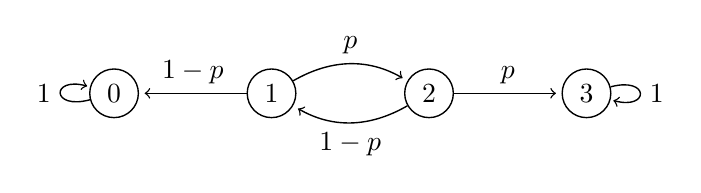
\begin{tikzpicture}[ - > , shorten >=2pt , line width =0.5 pt , node distance =2 cm]
			\node [circle , draw] (zero) {0};
			\node [circle , draw] (one) [right of=zero] {1};
			\node [circle , draw] (two) [right of=one] {2};
			\node [circle , draw] (three) [right of=two] {3};
			\path (zero) edge [loop left] node {$1$} (zero) ;
			\path (one) edge node [above] {$1 - p$} (zero) ;
			\path (one) edge [bend left] node [above]{$p$} (two) ;
			\path (two) edge node [above]{$p$} (three) ;
			\path (two) edge [bend left] node [below]{$1 - p$} (one) ;
			\path (three) edge [loop right] node {$1$} (three) ;
		\end{tikzpicture}
	\end{latin}
	\caption[یک مارکوف نمونه برای مسئله پاکباختگی]{یک زنجیره مارکوف نمونه برای مسئله پاکباختگی قمارباز\protect\footnotemark}
	\label{fig:gambler}
\end{figure}
\LTRfootnotetext{The Gambler's ruin}
\newpage
\begin{defi}
\label{def:two}
زنجیره مارکوف گسسته زمان $X(t)$ را \textbf{همگن-زمان} می‌گوییم اگر شرط زیر همواره برقرار باشد:
\begin{equation*}
P\left(X_{n+1}=j \mid X_{n}=i\right)=P\left(X_{1}=j \mid X_{0}=i\right)
\end{equation*}
به عبارت دیگر یعنی احتمالات مربوط به انتقال بین حالت‌ها به زمان \(t\) وابسته نیستند. در این حالت احتمال انتقال زنجیره از حالت \(i\) به \(j\) را با عبارت $p_{i j}=P\left(X_{1}=j \mid X_{0}=i\right)$ نمایش می‌دهیم و همچنین ماتریس انتقال را با $P=\left(p_{i j}\right)$ نمایش می‌دهیم. ماتریس انتقال را می‌توان به صورت یک گراف جهت‌دار نیز توصیف کرد به طوری که درایه $p_{i, j}$ در ماتریس معادل یک یال جهت‌دار از راس $i$ به راس $j$ با وزن $p_{i, j}$ است.
\end{defi}
طبق تعاریف \ref{def:one} و \ref{def:two} می‌توان زنجیره مارکوف گسسته‌زمانی برای حالت دستگاه کاربر در طی زمان در نظر گرفت که در آن حالت دستگاه کاربر $\tau[t]$ حالت زنجیره در زمان $t$ را مشخص می‌کند. همچنین ماتریس انتقال $\chi$ تعریف می‌شود به طوری که $\chi_{\tau, \tau^{\prime}}$ احتمال انتقال از حالت $\tau$ به \(\tau^{\prime}\) را مشخص می‌کند. \\

ماتریس انتقال را می‌توان به ازای یک استراتژی تخلیه داده شده و پارامترهای سیستمی مانند \(\alpha_1, \cdots, \alpha_k\) بدست آورد. در شکل \ref{fig:digraph} گراف جهت‌دار معادل زنجیره مارکوف برای یک سیستم با یک صف وظیفه و \(Q = 2\) و تعداد ۲ قسمت به ازای هر وظیفه و تعداد ۱ بسته به ازای هر وظیفه رسم شده است.\footnote{کد استفاده شده برای رسم این گراف در آدرس \lr{https://github.com/dalisyron/OffloadingVisualizer} موجود می‌باشد}
\begin{figure}[H]
\centering
\includegraphics[width=\textwidth]{figures/graph.pdf}
\caption[زنجیره مارکوف سیستم تخلیه در قالب گراف جهت دار]{
زنجیره مارکوف سیستم تخلیه در قالب گراف جهت دار (برای مشاهده جزئیات زوم کنید)
}
\label{fig:digraph}
\end{figure}
به منظور محاسبه معیارهایی مانند توان مصرفی میانگین و تاخیر سرویس میانگین لازم است که بتوانیم درباره وضعیت سیستم تخلیه وظیفه در طولانی‌مدت استنتاج کنیم. در همین راستا مفهوم توزیع پایدار را تعریف می‌کنیم.
\begin{defi}
به ازای یک زنجیره مارکوف داده شده با ماتریس انتقال \(P\) یک \textbf{توزیع پایدار} توزیع احتمالی مانند \(\pi\) است که شرط زیر برای آن برقرار باشد:
\begin{equation*}
	\pi=\pi P \quad \Longleftrightarrow \quad \pi_{j}=\sum_{i} \pi_{i} P_{i j} \quad \forall j .
\end{equation*}
\end{defi}
یک سوالی که ممکن است بوجود بیاید این است که آیا لزوما هر زنجیره مارکوف گسسته زمانی توزیع پایدار دارد؟ برای پاسخ به این سوال لازم است دو مفهوم زنجیره مارکوف تقلیل‌ناپذیر و غیرمتناوب را تعریف کنیم.
\begin{defi}
اگر رسیدن از هر نقطه به نقطه دیگر از فضای حالت با احتمال مثبت در زنجیره مارکوف میسر باشد، زنجیره را \textbf{تقلیل‌ناپذیر} گویند. به بیان ریاضی می‌توان تقلیل‌ناپذیر بودن زنجیره مارکوف را به صورت زیر نشان داد.
\begin{equation*}
	\operatorname{Pr}\left(X_{n_{i j}}=j \mid X_{0}=i\right)=p_{i j}^{\left(n_{i j}\right)}>0
\end{equation*}
\end{defi}

\begin{defi}
تناوب $d(i)$ برای حالت $i$ به صورت $d(i)=\operatorname{gcd}\left\{n: P_{i i}^{n}>0\right\}$ تعریف می‌شود، که به معنی بزرگ‌ترین مقسوم علیه مشترک تعداد مراحل ممکن است به صورتی که از $i$ شروع کرده و به $i$ برگردیم. یک زنجیره مارکوف تقلیل‌ناپذیر را متناوب با تناوب $d$ می‌گوییم اگر تمامی حالت‌ها تناوب $d > 1$ را داشته باشند. یک زنجیره مارکوف تقلیل ناپذیر را \textbf{غیرمتناوب} می‌گوییم اگر تمامی حالت‌ها تناوب برابر ۱ داشته باشند.
\end{defi}
\begin{thm}
\textbf{(همگرایی)}
هر زنجیره مارکوف تقلیل‌ناپذیر و غیر متناوب دارای توزیع پایدار منحصر به فردی مانند $\pi$ می‌باشد.
\end{thm}
حال با استفاده از قضیه ۳.۱. ثابت می‌کنیم که زنجیره مارکوف مربوط به سیستم تخلیه وظیفه دارای توزیع پایدار منحصر به فرد است. برای سادگی فرض می‌کنیم که سامانه یک صف دارد و سپس نحوه بسط نتیجه به چندین صف را توضیح می‌دهیم.

\begin{thm}
\label{thm:irreducible}
زنجیره مارکوف مربوط به سیستم تخلیه تک صف تقلیل ناپذیر است. \\
\textbf{اثبات:} \\
قسمت الف) با توجه به تعریف سیستم تخلیه می‌دانیم که از هر حالت غیر شروع مانند \( (0, 0, 0) \neq (x, y, z)\) می‌توان به حالت شروع رفت. به این منظور کافی است که تمام وظایف داخل صف به نحوی (اجرا یا ارسال) به اتمام برسند و وظیفه جدیدی نیز در این حین وارد سیستم نشود. \\

قسمت ب) همچنین می‌توان ثابت کرد که از حالت شروع \((0, 0, 0)\) می‌توان به هر حالت دیگر \((x, y, z)\) رفت. به این منظور دنباله رخدادهای زیر را در نظر بگیرید:
\begin{enumerate}
	\item ورود \(x\) وظیفه جدید
	\item انتقال یک وظیفه به واحد ارسال و ورود یک وظیفه جدید، هر دو در صورتی که \(y > 0\)
	\item پیشرفت واحد ارسال به مدت \(y\) سیکل و عدم ورود وظیفه جدید در این حین
	\item انتقال یک وظیفه به پردازنده و ورود یک وظیفه جدید، هر دو در صورتی که \(z > 0\)
	\item پیشرفت واحد ارسال به مدت \(z\) سیکل و عدم ورود وظیفه جدید در این حین
\end{enumerate}
با توجه به نتایج بخش الف و ب می‌توان نتیجه گرفت که از گشتی با احتمال مثبت از هر حالت به حالت دیگر وجود دارد بنابراین طبق تعریف زنجیره تقلیل‌ناپذیر است.
\end{thm}
\begin{thm}
\label{thm:aperiodic}
زنجیره مارکوف مربوط به سیستم تخلیه تک صف غیر متناوب است. \\
\textbf{اثبات:} \\
به منظور اثبات این قضیه فقط کافی است که به این نکته توجه کنیم که در زنجیره حالت \((0, 0, 0)\) دارای تناوب یک می‌باشد. زیرا با احتمالی مثبت (متناظر با رخداد عدم ورود وظیفه و کنش \lr{No Operation}) می‌توان در همان حالت ماند. با توجه به همین نکته و تقلیل‌ناپذیر بودن زنجیره میتوانیم نتیجه بگیریم که سایر حالت‌ها نیز باید تناوب یک داشته باشند. بنابراین زنجیره غیرمتناوب است.
\end{thm}
با توجه به قضایای \ref{thm:irreducible} و \ref{thm:aperiodic} و قضیه همگرایی می‌توان نتیجه گرفت که زنجیره مارکوف سیستم تخلیه تک صف دارای توزیع پایدار منحصر به فرد می‌ مطابق با رابطه \ref{eq:steady} می‌باشد. برای بسط این اثبات به حالت چند صف اثبات غیرمتناوب بودن یکسان خواهد بود و در اثبات تقلیل‌ناپذیر بودن، رخداد اول به ورود \(x_1, \cdots, x_k\) وظیفه از انواع مختلف تغییر پیدا می‌کند.
\begin{equation}
	\label{eq:steady}
	\left\{\begin{array}{l}
		\sum_{\boldsymbol{\tau}^{\prime} \in \mathcal{S}} \chi_{\boldsymbol{\tau}^{\prime}, \boldsymbol{\tau}} \pi_{\boldsymbol{\tau}^{\prime}}=\pi_{\boldsymbol{\tau}}, \forall \boldsymbol{\tau} \in \mathcal{S} \\
		\sum_{\boldsymbol{\tau} \in \mathcal{S}} \pi_{\boldsymbol{\tau}}=1
	\end{array}\right.
\end{equation}
\section{محاسبه تاخیر میانگین}
تاخیر هر وظیفه شامل تاخیر انتظار در صف وظایف و تاخیر پردازش می‌باشد. به منظور بدست آوردن تاخیر میانگین سیستم ابتدا $\theta_i$ را به عنوان کسری از وظایف سیستم در طولانی مدت که از نوع $i$ هستند تعریف می‌کنیم. اگر طول صف‌ها به مقدار کافی بزرگ باشد و همچنین استراتژی تخلیه‌ای داشته باشیم که منجر به پر شدن صف و اتلاف وظیفه\LTRfootnote{Task Loss} نشود مقدار $\theta_i$ طبق رابطه \ref{eq:theta} بدست می‌آید.
\begin{equation}
\label{eq:theta}
\theta_i = \frac{\alpha_i}{\sum_{j=1}^{k} \alpha_{j}}
\end{equation}
\newpage
پارامتر \(t_q^i\) را برابر با مقدار میانگین تاخیر انتظار در صف مربوط به وظایف نوع $i$ تعریف می‌کنیم. طبق قانون \lr{Little} می‌توان مقدار این تاخیر را بر اساس رابطه \ref{eq:queuing-delay} بدست آورد. همانطور که پیش‌تر ذکر شد برای برقراری این رابطه لازم است که اتلاف وظیفه در صف هیچ‌گاه رخ ندهد. به عبارت دیگر با فرض اینکه استراتژی تخلیه‌ی ارائه شده «کارامد» باشد این رابطه برقرار است. در پیاده‌سازی عملی، محدودیت «کارآمد» بودن یک استراتژی بدین گونه تعریف شده است که احتمال پر بودن صف حداکثر مقداری ناچیز  باشد.

\begin{equation}
	\label{eq:queuing-delay}
	t_{q}^i=\frac{\theta_i}{\alpha_i} \sum_{j=0}^{Q} i \cdot \operatorname{Pr}\{q_i[t]=i\}=\frac{1}{\alpha} \sum_{\tau \in S} \tau\{q_i\} \cdot \pi_{\tau}
\end{equation}
همچنین $t_{tx}^i$ را به عنوان تاخیر ارسال میانگین یک وظیفه از نوع \(i\) توسط واحد ارسال تعریف می‌کنیم که مقدار آن بر اساس امید ریاضی موفقیت در فرآیند برنولی مطابق با رابطه \ref{eq:bernouli} بدست می‌آید.
\begin{equation}
	\label{eq:bernouli}
	t_{t x}^i=M_i \sum_{j=1}^{\infty} j(1-\beta)^{(j-1)} \beta
\end{equation}
به یاد داریم که مقدار تاخیر در صورت پردازش محلی برای وظایف نوع $i$ برابر $L_i$ می‌باشد. تاخیر اجرا در صورت تخلیه وظیفه به صورت مجموع زمان ارسال وظیفه
$t_{tx}^i$
زمان اجرا در سرور لبه‌ای
$C_i$
و تاخیر دریافت نتیجه از سرور
$t_{rx}^i$
محاسبه می‌شود.
\begin{equation}
	t_{c}^i=t_{t x}^i+C_i+t_{rx}
\end{equation}
در نتیجه می‌توان تاخیر اجرای میانگین وظایف نوع $i$ را نیز مطابق رابطه \ref{eq:proc-delay} بیان کرد.
\begin{equation}
	\label{eq:proc-delay}
	t_{p}^i=\eta_i L_i+(1-\eta_i) t_{c}^i
\end{equation}
که در آن
$\eta_i$
بیانگر کسری از وظایف نوع $i$ می‌باشد که در طولانی‌مدت به صورت محلی اجرا می‌شوند و مطابق با رابطه \ref{eq:eta} بدست می‌آيد.
\begin{equation}
	\label{eq:eta}
	\eta_i=\frac{\sum_{\boldsymbol{\tau, a} \in \mathcal{S}_{1}^i\cup\mathcal{S}_{3}^i\cup\mathcal{S}_{5}^i} \pi_{\boldsymbol{\tau}} g_{\boldsymbol{\tau}}^{a} }{\sum_{\boldsymbol{\tau, a} \in \mathcal{S}_{1}^i\cup\mathcal{S}_{2}^i\cup\mathcal{S}_{3}^i\cup\mathcal{S}_{4}^i} \pi_{\boldsymbol{\tau}} g_{\boldsymbol{\tau}}^{a} + 2 \sum_{\boldsymbol{\tau, a} \in S_5^i} \pi_{\boldsymbol{\tau}} g_{\boldsymbol{\tau}}^{a}}
\end{equation}
که در آن
$S_1^i, \cdots, S_5^i$
به صورت زیر تعریف می‌شوند:
\begin{equation}
	\begin{aligned}
		& S_1^i = \{\boldsymbol{\tau, a} \in \mathcal{S} \times A | type(a) = AddToCPU \land locType(a) = i\} \\
		& S_2^i = \{\boldsymbol{\tau, a} \in \mathcal{S} \times A | type(a) = AddToTU \land offloadType(a) = i\} \\ 
		& S_3^i = \{\boldsymbol{\tau, a} \in \mathcal{S} \times A | type(a) = AddToBoth \land locType(a) = i \land offloadType(a) \neq i\} \\
		& S_4^i = \{\boldsymbol{\tau, a} \in \mathcal{S} \times A | type(a) = AddToBoth \land locType(a) \neq i \land offloadType(a) = i\} \\
		& S_5^i = \{\boldsymbol{\tau, a} \in \mathcal{S} \times A | type(a) = AddToBoth \land locType(a) = i \land offloadType(a) = i\}
	\end{aligned}
\end{equation}
در رابطه فوق تابع $type(a)$ نوع کنش را مشخص می‌کند و یکی از چهار نوع بیان شده در بخش \ref{sec:action} می‌باشد. توابع
$locType(a)$
و
$offloadType(a)$
نیز نوع وظیفه مربوط به کنش $a$ را مشخص می‌کنند. \\

با استفاده از روابط بالا همچنین می‌توانیم میانگین تاخیر سرویس هر وظیفه در سیستم را طبق رابطه \ref{eq:total-delay} محاسبه کنیم. نکته مهم این است که این تابع همان تابع هدف برای کمینه‌سازی در مسئله پیدا کردن استراتژی تخلیه بهینه است.
\begin{equation}
	\label{eq:total-delay}
	\bar{T}=\sum_{i=1}^{k} \theta_{i}\left(t_{q}^{i}+t_{p}^{i}\right)
\end{equation}
\newpage
\section{توان مصرفی میانگین}
اگر پارامتر
$\mu_\tau^{loc}$
و 
$\mu_\tau^{tx}$
را که به ترتیب به عنوان احتمال فعالیت پردازنده در حالت
$\tau$
و احتمال فعالیت واحد ارسال در حالت
$\tau$
تعریف کنیم، آنگاه توان مصرفی میانگین طبق رابطه زیر بدست می‌آید:
\begin{equation}
	\bar{P}=\sum_{\boldsymbol{\tau} \in \mathcal{S}} \pi_{\boldsymbol{\tau}}\left(\mu_{\boldsymbol{\tau}}^{l o c} P_{l o c}+\mu_{\boldsymbol{\tau}}^{t x} P_{t x}\right)
\end{equation}

\section{استراتژی تخلیه وظیفه بهینه}
با توجه به توابع بدست آمده برای تاخیر و توان مصرفی میانگین در بخش‌های پیشین، حال می‌توانیم مسئله پیدا کردن استراتژی تخلیه بهینه را به صورت یک مسئله بهینه سازی مانند
$\mathcal{P}_{1}$
بیان کنیم:
\begin{equation}
		\begin{aligned}
			\mathcal{P}_{1}: \min _{\left\{g_{\tau}^{a}\right\}}\; & \bar{T} = (\sum_{i=1}^{k} \frac{1}{\alpha_i} \sum_{\tau \in S} \tau\{q_i\} \cdot \pi_{\tau}) + T_p^0 \\
			\text { \lr{s.t.} } &\left\{\begin{array}{l}
				\bar{P} \leq \bar{P}_{\max } \\
				\sum_{\boldsymbol{\tau}^{\prime} \in \mathcal{S}} \chi_{\boldsymbol{\tau}^{\prime}, \boldsymbol{\tau}} \pi_{\boldsymbol{\tau}^{\prime}}=\pi_{\boldsymbol{\tau}}, \boldsymbol{\tau} \in \mathcal{S}, \\
				\sum_{\boldsymbol{\tau} \in S} \pi_{\boldsymbol{\tau}}=1, \\
				\sum_{\alpha \in A} g_{\tau}^{\alpha}=1, \forall \tau \in S\\
				g_{\tau}^{a} \geq 0, \forall \tau \in S,\;a \in A
			\end{array}\right.
		\end{aligned}
\end{equation}
که در آن
$T_p^0$
برابر با تاخیر اجرای میانگین است که به ازای مقادیر داده شده از
$\eta_0, \cdots, \eta_k$
مقداری ثابت دارد و از رابطه زیر بدست می‌آید:
\begin{equation}
	T_p^0 = \sum_{i=1}^{k} (\eta_i L_i+(1-\eta_i) t_{c}^i)
\end{equation}
\clearpage
با توجه به وجود پارامتر $\eta_i$ در تابع هدف
$\mathcal{P}_{1}$
این مسئله بهینه‌سازی، یک مسئله خطی نیست. با این حال می‌توانیم با استفاده از تغییری کوچک مسئله را به دنباله‌ای از مسائل برنامه‌ریزی خطی تبدیل کنیم. به این منظور مشابه \cite{Liu} از تعریف «معیار احاطه\LTRfootnote{Occupation Measure}» در زنجیره مارکوف استفاده می کنیم. به طور دقیق‌تر مجموعه متغیرهای جدید $\left\{x_{\tau}^{a}\right\}$ را تعریف می‌کنیم به طوری که  $x_{\tau}^{a}=\pi_{\tau} g_{\tau}^{a}$ تعریف می‌کنیم. به عبارتی $x_{\tau}^{a}$ برابر با احتمال حضور در حالت $\tau$ و انتخاب کنش
$a$
می‌باشد. همچنین طبق تعریف 
$\sum_{a \in A} g_{\tau}^{a}=1$
و بنابراین
$\pi_{\boldsymbol{\tau}}=\sum_{a \in A} x_{\boldsymbol{\tau}}^{a}$
\\\\
حال با جایگذاری $\left\{x_{\tau}^{a}\right\}$ به جای $\{\pi_\tau\}$ در
$\mathcal{P}_{1}$
خواهیم داشت:
\begin{equation}
	\begin{aligned}
		\mathcal{P}_{2}: \min _{\boldsymbol{x}, \eta}\; & \bar{T}=(\sum_{i=1}^{k} \frac{1}{\alpha_i} \sum_{\tau \in \mathcal{S}} \sum_{a \in A} \tau\{q_i\} \cdot x_{\tau}^{a})+ T_p^0 \\
		\text { \lr{s.t.} } &\left\{\begin{array}{l}
			\nu_{l o c}(\boldsymbol{x}) P_{l o c}+\beta \nu_{t x}(\boldsymbol{x}) P_{t x} \leq \bar{P}_{\max } \\
			\Gamma(\boldsymbol{x}, \eta_i)=, \forall i \in \{1, \cdots, k\}\\
			F_{\tau}(\boldsymbol{x})=0, \forall \tau=(i, m, n) \in \mathcal{S} \\
			\sum_{\tau \in \mathcal{S}} \sum_{a \in A}=1 \\
			\eta_i \in [0, 1], \forall i \in \{1, \cdots, k\} \\
			x_{\tau}^{a} \geq 0, \forall \tau \in S, a \in A
		\end{array}\right.
	\end{aligned}
\end{equation}
که در آن
$\nu_{l o c}$
و
$\nu_{t x}$
به ترتیب احتمال فعالیت پردازنده و واحد ارسال را در یک واحد زمانی دلخواه مشخص می‌کنند و به ازای یک استراتژی داده شده قابل محاسبه اند. \footnote{برای مشاهده روش محاسبه این دو پارامتر در قالب کد به پیوست ۲ مراجعه شود.} تابع
$\Gamma(\boldsymbol{x}, \eta_i)$
بر اساس رابطه \ref{eq:eta} می‌باشد و به صورت زیر محاسبه می‌شود:
\begin{equation}
	\Gamma(x, \eta) = \eta  \sum_{\boldsymbol{\tau, a} \in \mathcal{S}_{1}^i\cup\mathcal{S}_{2}^i\cup\mathcal{S}_{3}^i\cup\mathcal{S}_{4}^i} x_{\tau}^a + 2 \eta \sum_{\boldsymbol{\tau, a} \in S_5^i} x_{\tau}^a
	- \eta \sum_{\boldsymbol{\tau, a} \in \mathcal{S}_{1}^i\cup\mathcal{S}_{3}^i\cup\mathcal{S}_{5}^i} x_{\tau}^a
\end{equation}
و تابع 
$F_{\tau}(\boldsymbol{x})$
به صورت زیر تعریف می‌شود:
\begin{equation}
	F_{\tau}(\boldsymbol{x})=\sum_{\tau^{\prime} \in \mathcal{S}} \sum_{a \in A} \tilde{\chi}_{\tau^{\prime}, \tau, a} x_{\tau^{\prime}}^{a}-\sum_{a \in A} x_{\tau}^{a}
\end{equation}
در رابطه فوق منظور از
$ \tilde{\chi}_{\tau^{\prime}, \tau, a}$
احتمال این است که به شرط اینکه در حالت
$\tau^{\prime}$
باشیم و کنش
$a$
انتخاب شده باشد، آنگاه به حالت
$\tau^{\prime}$
برویم. \\

در صورتی که مقادیر
$\eta_0, \cdots, \eta_k$
معلوم باشد آنگاه مسئله
$\mathcal{P}_2$
تبدیل به یک مسئله برنامه‌ریزی خطی می‌شود. با یافتن مقادیر جواب بهینه
$\left\{x_{\tau}^{a}\right\}$ 
می‌توان استراتژی بهینه را طبق رابطه زیر بدست آورد:
\begin{equation}
	g_{\tau}^{a *}=\frac{x_{\tau}^{a *}}{\sum_{a \in A} x_{\tau}^{a *}}, \forall \tau \in \mathcal{S}, a \in A
\end{equation}
بنابراین جهت یافتن استراتژی بهینه برای یک سیستم تخلیه وظیفه کافی است که مسئله برنامه‌ریزی خطی حاصل از
$\mathcal{P}_2$
را به ازای مقادیر مختلف 
$\eta_0, \cdots, \eta_k$
حل کرده تا استراتژی بهینه بدست بیاید. مراحل این فرآیند جستجو در الگوریتم ۱ به صورت خلاصه آمده است.

\begin{latin}
	\begin{algorithm}
		\rl{\caption{الگوریتم جستجوی استراتژی تخلیه وظیفه بهینه}}\label{alg:cap}
		\begin{algorithmic}[1]
			\Require $precision \geq 2$
			\State $etaSettings \gets splitRange([0, 1], precision)^k$
			\State $optimalPolicy = null$
		    \ForEach {$s \in etaSettings$}
				\State $(\eta_0, \cdots, \eta_k) \gets s$
				\State $solution \gets solveLP(\eta_0, \cdots, \eta_k)$
				\If{$optimalPolicy = null\;\mathbf{or}\;solution.delay < optimalPolicy.delay$}
					\State $optimalPolicy \gets solution.policy$
				\EndIf
			\EndFor \\
			\Return $optimalPolicy$
		\end{algorithmic}
	\end{algorithm}
\end{latin}